\begin{figure*}[h]
\centering
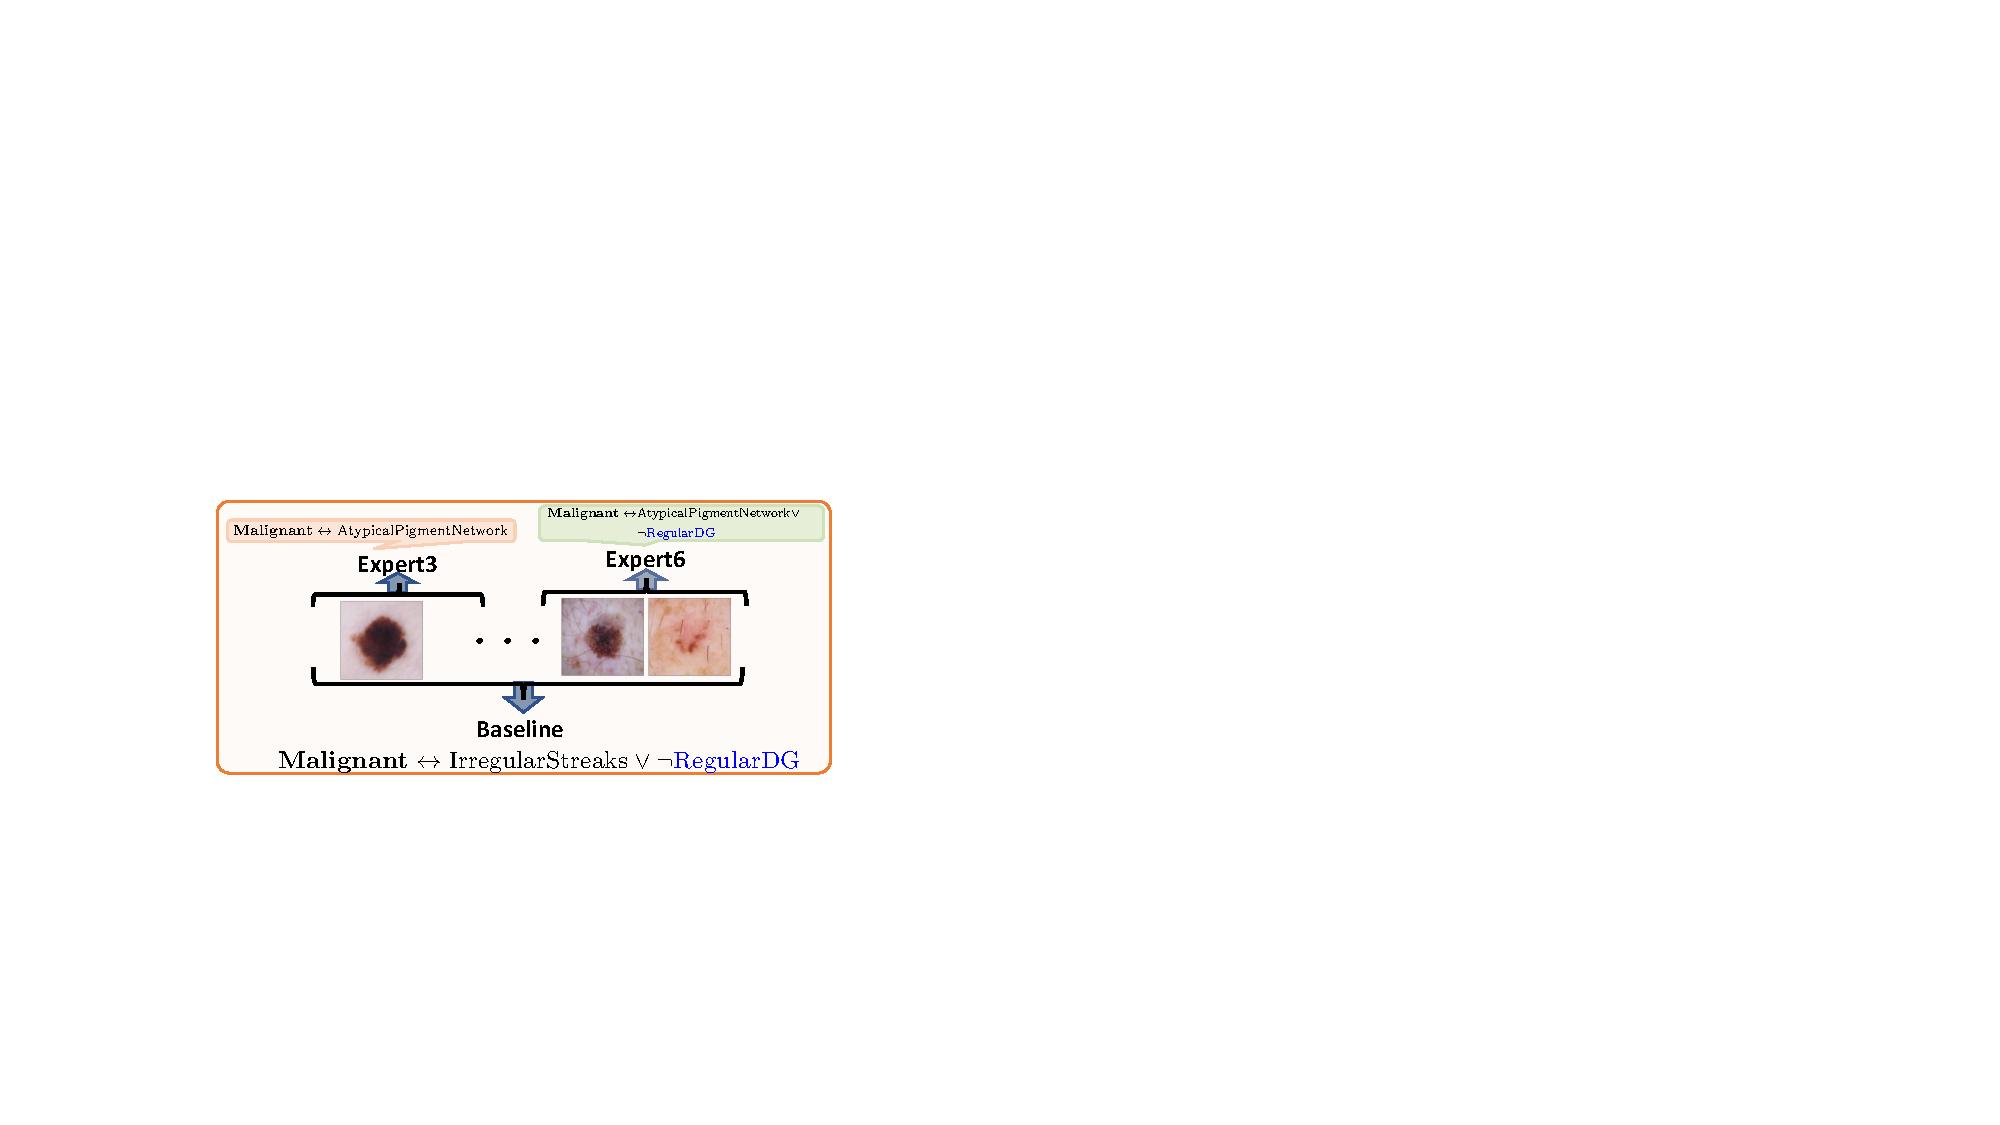
\includegraphics[width=\columnwidth]{figures/Supp/Local_isic.pdf}
\vspace{-10pt}
\caption{Flexibility of FOL explanations by VIT-derived MoIE  MoIE and  the baselines for Awa2 dataset. We compare the FOL for different MoIE experts with the baselines to classify (a) Otter (b) Horse in Awa2For example in figure (b), the baseline's FOL constitutes identical concepts to distinguish all the samples ``Horse''. However, expert4 classifies ``Horse'' with \textit{smelly} as the identifying concept for the instances covered by it. Similarly expert5 classifies the same ``Horse'' using \textit{longneck} and \textit{fields}.  We highlight the shared concepts between the experts and the baselines.}
\label{fig:local_awa2}
\vspace{-2.5pt}
\end{figure*}

xxxxx